%!TEX root = main.tex

% =============================================================================
\section{Introduction}
\label{sec:introduction}
% =============================================================================

\begin{figure}[t]
    \centering
    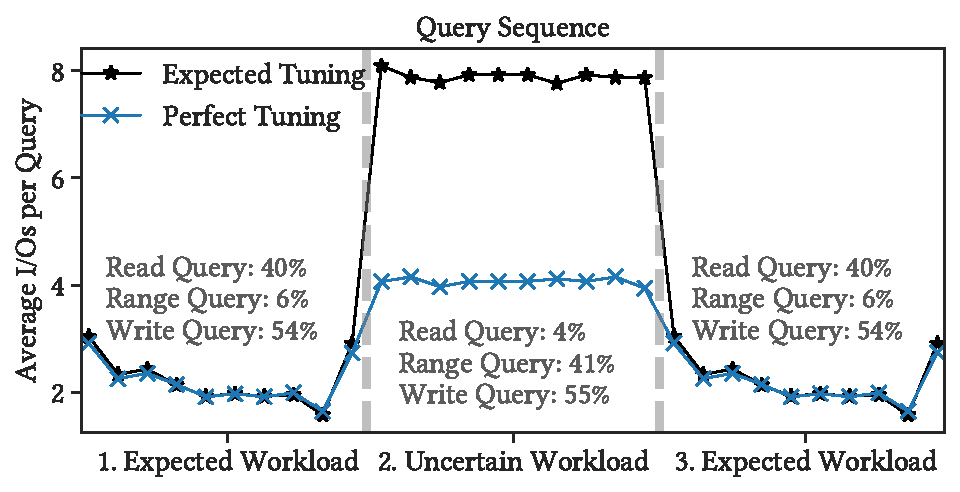
\includegraphics[scale=0.5]{figures/introduction_sequence.pdf}
    \caption{LSM tree tunings and their performance on observed workloads. While
        both workloads have a similar ratio of reads and writes, the uncertain
        workload has a higher percentage of range queries leading to the
        expected system tuning to experience a $2\times$ degradation in
        performance.}
    \label{fig:introduction_query_seq}
\end{figure}

\Paragraph{Ubiquitous LSM-based Key-Value Stores}
Log-Structured Merge trees (LSM trees) is the most commonly deployed data structure
used in the backend storage of modern key-value stores~\cite{ONeil1996}.
LSM trees offer high ingestion rate and fast reads,
    making them widely adopted by systems such as RocksDB~\cite{FacebookRocksDB} 
    at Facebook, LevelDB~\cite{GoogleLevelDB} and BigTable~\cite{Chang2006} at 
    Google, HBase~\cite{HBase2013} and Cassandra~\cite{ApacheCassandra} at 
    Apache, WiredTiger~\cite{WiredTiger} at MongoDB, X-Engine \cite{Huang2019} 
    at Alibaba, and DynamoDB~\cite{DeCandia2007} at Amazon.
           
LSM trees store incoming data in a memory buffer, which 
    is flushed to storage when it is full and merged with
    earlier flushed buffers to form a collections of sorted runs 
    with exponentially increasing sizes~\cite{Luo2020b}. 
Frequent merging of sorted runs leads to higher merging costs, but facilitates
    faster lookups (\emph{leveling}).
On the flip side, lazy merging policies (\emph{tiering}) trade lookup 
    performance for lower merging costs~\cite{Sarkar2021c}.
Maintaining a separate Bloom filter~\cite{Bloom1970} per sorted run 
    optimizes point query throughput by avoiding unnecessary accesses to runs 
    that do not contain the desired data.
Range query performance, while not benefiting from the presence of traditional 
    Bloom filters, depends on the LSM tree structure.  
   
% Merging sorted runs can happen eagerly, leading to higher merging cost but 
%     faster lookups (\emph{leveling}), or lazily, leading to lower merging cost 
%     but slower lookups (\emph{tiering})~\cite{Sarkar2021c}. 
% Point queries are supported by a Bloom filter (Bloom filter)~\cite{Bloom1970}
%     per sorted run to avoid unnecessary accesses to runs that
%     do not contain the desired data. 
% \Paragraph{Tuning LSM trees}

\Paragraph{Tuning LSM trees} Increasing number of applications relying on LSM-based storage
    backends, has brought a lot of attention to the problem of  of tuning LSM trees for optimal performance.     
The common characteristic of all these methods, is the \emph{assumption that one has full knowledge of
the expected workload and of
the underlying system 
    resources} (processing units, memory, storage).
    Given such knowledge, there are a lot of works that optimize memory allocation to Bloom filters across different levels, 
memory distribution between buffers and Bloom filters and merging policies (i.e.,  \emph{leveling} or \emph{tiering})~\cite{Dayan2017,Dayan2018a}.  
%We provide a detailed review of all these works in the Related Work section (see Section~\ref{sec:related_work}). 
Further LSM optimization efforts have lead to
hybrid merging policies to allow for more fine-grained 
tunings~\cite{Dayan2018,Dayan2019,Idreos2019}, optimized memory allocation 
strategies~\cite{Bortnikov2018,Kim2020,Luo2020a}, variations of Bloom 
filters~\cite{Luo2020,Zhang2018a,Zhang2020a}, new compaction 
routines~\cite{Alkowaileet2020,Luo2019a,Sarkar2020,Zhang2020}, and
exploitation of data characteristics~\cite{Yang2020, Ren2017, Absalyamov2018}.



% \iffalse
% A key avenue for optimization involves allocating appropriate memory for Bloom filters 
%     across different levels ~\cite{Dayan2017} %so that the levels responsible for highest
%    % number of unnecessary disk accesses have the largest Bloom filters
%     %~\cite{Dayan2017}. 
% Furthemore, knowledge about expected workloads is leveraged to
%     optimize memory distribution between buffers and Bloom filters while simultaneously
%     picking the optimal merging policy viz., \emph{leveling} or \emph{tiering}
%     ~\cite{Dayan2018a}.
% % Furthermore, using workload knowledge, a holistic tuning approach co-tunes the memory
% % allocation between the buffer and Bloom filters along with the 
% % merging policy (\emph{leveling} or \emph{tiering}) \cite{Dayan2018a}.
% Hybrid merging policies have been proposed to allow for more 
%     fine-grained tunings~\cite{Dayan2018,Dayan2019,Idreos2019}. 
% Additionally, optimized memory allocation strategies
%     ~\cite{Bortnikov2018,Kim2020,Luo2020a}, variations of Bloom filters
%     ~\cite{Luo2020,Zhang2018a,Zhang2020a}, application specific compaction 
%     routines~\cite{Alkowaileet2020,Luo2019a,Sarkar2020,Zhang2020}, and
%     exploitation of data characteristics~\cite{Yang2020, Ren2017, Absalyamov2018},
%     etc., have all contributed to recent advances in the field.
% % which pages to 
% % prefetch \cite{Yang2020}, exploiting semi-sorted data \cite{Ren2017}, and 
% % cardinality estimation \cite{Absalyamov2018}.
% \fi

% \Paragraph{Tuning \emph{Certainties} \& \emph{Uncertainties}}
\Paragraph{The Only Certainty is Uncertainty}
Even when accurate information about the workload and underlying hardware is 
available, tuning data systems in general is a notoriously difficult research 
problem \cite{Chaudhuri2004a,Chaudhuri2005,Shasha2002}. The explosive
growth in the public and private use of the cloud infrastructure for data
management~\cite{Hayes2008,Intel2011,GrandViewResearch2019} exacerbates the 
problem because it increases the uncertainty and the variability of the 
workloads~\cite{Chohan2010,Galante2012,Herbst2013,Holze2010,Mohan2016,Ozcan2017,Pezzini2014,Schnaitter2006,Schnaitter2007,
    Schnaitter2012,Wolski2017}. 
    
    
%     \iffalse
%     ~\cite{Chaudhuri2004a,Chaudhuri2005,Shasha2002}. 
% Recent explosive growth in the public \cite{Hayes2008} and private use of the 
%     cloud infrastructure systems~\cite{Intel2011,GrandViewResearch2019} has
%     made tuning even more challenging -- 
%     (i) workloads are hybrid~\cite{Mohan2016,Ozcan2017,Pezzini2014}, 
%     (ii) vary frequently
%     ~\cite{Holze2010,Schnaitter2006,Schnaitter2007,Schnaitter2012}, and 
%     (iii) dynamic resource availability due to prevalence of 
%     virtualization~\cite{Chohan2010,Galante2012,Herbst2013,Wolski2017}.
%     \fi
%
%More specifically, the typical assumptions that (a) we have trustworthy information about
%the expected workload that can be used to tune the system, (b) the available resources are known 
%a priori, (c) the hardware can be fully controlled by the system being tuned, (d) there is a sample 
%workload to be used for calibrating the system, and (e) the main metric to optimize is workload 
%performance, do not always hold when considering modern cloud deployments. 
%Resources are elastic, meaning that they 
%can scale up or down and in some cases even without guarantees 
%(depending on the pricing scheme) \cite{Chohan2010,Galante2012,Herbst2013,Wolski2017}.
%

% To account for such uncertainties, new metrics such as  
%     worst-case performance~\cite{Mozafari2015}, write and space 
%     amplification~\cite{Athanassoulis2016,Dong2017}, etc., are used in addition
%     to maximizing performance.

\Paragraph{An Example}  Before we describe our framework, we give an example that demonstrates how
variation in the observed workloads relative to the expected workload -- used to tune an LSM tree-based storage system --
leads to suboptimal performance. 
% Specifically, following prior work we consider a tuning paradigm where the 
%     tuner receives information about the expected workload, and uses this 
%     information to ascertain the best tuning with respect the memory allocation 
%     and the merging frequency and strategy for the underlying LSM-based 
%     storage backend. 
% If the observed workloads, however, differ from the expected workload the 
%     tuning is typically suboptimal. 
Figure ~\ref{fig:introduction_query_seq} shows a sequence of 
    workloads executed over an LSM-based engine. 
The $x$-axis is denotes a sequence of workloads and the $y$-axis shows the average 
    disk accesses per workload. 
The experiment is split in three sessions, where the first and the last sessions 
    receive the expected workloads,
    while the second session receives a different workload.
Although it has the same read-to-write ratio of queries as the expected 
    workload, it has a higher percentage of short range queries in comparison
    to the point queries.
% Both short range queries and point queries access only one page per 
% level. 
The solid black line shows the performance of a system tuned for the expected 
    workload. 
Note that average I/Os increase dramatically in the second session 
    although the amount of data being read is approximately the same.
% even though the actual data read is virtually the same. 
On the other hand, the blue line corresponds to
each session having its ideal tuning, leading to only half as many I/Os per operation.
Note that it is not feasible to change tunings during execution as it would require
redistributing the allocated memory between different components of the tree and
potentially changing the shape of the tree. Rather, we want to \emph{find a 
tuning that is close-to-optimal for both the expected and the observed 
workload}.

    
\Paragraph{Our Work: Robust LSM Tree Tuning}    
To address the suboptimal system performance due to the variability in the observed workloads, we depart
from the classical view of database tunings which assumes that the expected workload is known. Rather, 
we incorporate uncertainty into our workload and we introduce {\it Endure} a new \emph{robust tuning paradigm} and we 
apply it to LSM trees.
%To address this issue, our work aims to offer a tuning approach that provides
%    a reliably high performance when faced with dynamic workloads, while 
%    sacrificing minimal performance in absence of uncertainty.
% An ideal solution is to switch to the best tuning per session, however, this is not feasible. Since a
% different LSM tuning may require reallocating memory between the buffer and the 
% Bloom filters, and changing merging frequency or policy, applying a different tuning would 
% typically require to stop and restart the system. 
% Instead, we want to find
% a tuning that can be used across all sessions, which can offer close-to-optimal
% performance when we execute a workload that is not identical with the one 
% used to tune, and that has low to no penalty when we received the expected
% workload. 
We propose a formulation that asks for the LSM tree configuration that maximizes the worst-case throughput over all the 
workloads in the \emph{neighborhood} of an expected workload. We call this problem 
the {\robustw} problem. We use the notion of KL-divergence between probability 
distributions to define the size of this neighborhood, implicitly 
assuming that the uncertain workloads would likely be contained in the 
neighborhood. As the KL-divergence boundary condition approaches zero, 
our problem becomes equivalent to the classical optimization problem (termed, 
the {\nominal} problem). More specifically, our approach uses as input the expected 
size of the uncertainty neighborhood, which dictates the qualitative 
characteristics of the solution. Intuitively, the larger the uncertainty
region considered, the larger workload discrepancy robust tuning can absorb.
Leveraging  work on robust optimization from the Operations Research 
community~\cite{Bertsimas2010, Ben-Tal1998, Ben-Tal2013}, we are able to efficiently solve the 
{\robustw} problem and find the robust tuning for LSM tree-based storage systems.
    

% of looking for the tuning that minimizes the 
% execution cost of the expected workload, we create a new optimization formulation
% that is looking for the tuning that minimize the worst-case execution cost when
% the workload is in a \emph{neighborhood} of the expected workload. To do this we
% define the \emph{uncertainty region} of the input workload, and the tuning now
% depends on the expected workload and the size of its uncertainty region. 
% Intuitively, when the size of the uncertainty region is zero our robust tuning
% formulation is identical to the classical tuning problem. However, as we increase
% the uncertainty region we can be close-to-optimal in cases that the observed 
% workload differs from the expected one. In order to define the \emph{uncertainty region} ... \mynote{a few sentences on how to define the \emph{uncertainty region}}
%
\Paragraph{Contributions}
To the best of our knowledge, our work presents the first systematic approach
    for robust tuning of LSM tree-based key-value stores under workload uncertainty. 
%
%Equiped with the correct formulation of the robust database tuning problem,
%    any one of the commercially available as well as open source non-linear
%    constrained optimization libraries can be used to obtain tunings that are
%    robust to variations in workloads.
% We develop a new tuner using \textcolor{red}{which solver?} 
% and we integrate it to RocksDB \cite{FacebookRocksDB} a state-of-the-art
% LSM-based storage engine. 
Our technical and practical contributions can be summarized as follows: %main contributions are as follows, 
%\begin{itemize}
\squishlist
	\item We incorporate workload uncertainty into LSM tuning and motivated by 
	problem definitions in the operations-research community we formulate the {\robustw} problem.  
	\item Our problem formulation can be meta-tuned to a specific degree of uncertainty in the expected workload.
%	\item We propose a representation of the uncertainty w.r.t. an expected 
%        workload that allows the robust formulation to target a specific 
%        degree of uncertainty.
	% \item We develop a solution \mynote{1 sentence about the solver and how it workds} 
	\item Leveraging results from the operations-research community, we show that we can find a robust LSM tuning efficiently. Our algorithm is also easy to implement in practice.
    \item We augment the existing analytical cost models of LSM tree-based storage systems
        with more precise methods to compute costs of workload execution.
      % and 
       % further integrate an open source non-linear optimizer into them for 
       % the purpose of robust tuning. 
	\item We show that robust tuning matches classical tuning when there is 
        no uncertainty, while providing up to 95\% higher throughput
        on average when faced with uncertain workloads.
	\item We integrate the proposed framework in RocksDB, a state-of-the-art LSM-based engine, and we validate the performance benefits of our robust tunings.
    \item We make our robust tuning framework publicly available to encourage
        reproducible research~\cite{github-repo}.
	% \item We experimentally observe that robust tuning leads to ... \mynote{add a high-light result from the systems experiments}
%\end{itemize}
\squishend
